\documentclass{article}

\usepackage{microtype}
\usepackage{graphicx}
\usepackage{booktabs}
\usepackage{xcolor}
\usepackage{listings}
\usepackage{hyperref}
\usepackage{url}
\usepackage{amssymb}
\usepackage{amsmath}
\usepackage{enumitem}
\usepackage{balance}

\newcommand{\theHalgorithm}{\arabic{algorithm}}
\usepackage[accepted]{icml2025}

\icmltitlerunning{PAD: Stateless Brain, Stateful Hub for Agent Fleets}

\usepackage{tikz}
\usetikzlibrary{positioning,arrows.meta,shapes.geometric,fit,backgrounds}

\hypersetup{
  colorlinks=true,
  linkcolor=black,
  citecolor=black,
  urlcolor=blue!55!black,
}

\usepackage{fancyvrb}
\usepackage{tcolorbox}

\begin{document}

\icmltitle{PAD: Separating the Stateless Brain from the Stateful Hub\\for Heterogeneous Long-Horizon Agent Fleets}

\begin{icmlauthorlist}
\icmlauthor{Yanming Liu}{zju}
\icmlauthor{Xinyue Peng}{seu}
\end{icmlauthorlist}

\icmlcorrespondingauthor{Yanming Liu}{oceann24@zju.edu.cn}
\icmlcorrespondingauthor{Xinyue Peng}{xinyuepeng@seu.edu.cn}

\icmlaffiliation{zju}{Zhejiang University, Hangzhou, China}
\icmlaffiliation{seu}{Southeast University, Nanjing, China}

\icmlkeywords{agent harness, long-horizon tasks, task orchestration, capability routing,
  state externalization, Model Context Protocol, verification}

\vskip 0.3in
\printAffiliationsAndNotice{}

% ============================================================ ABSTRACT
\begin{abstract}
Long-horizon agent systems fail not because the model cannot reason, but because the
\emph{runtime} loses track of what was asked, what has been done, and what counts as
evidence that it was done. Recent harness work attacks this by putting more into the
context window---bigger prompts, longer transcripts, recursive subagents---and by
adding more capability to a single execution environment. We argue the opposite
direction is what scales: \textbf{move all durable state out of the model and out of
the execution environment}, and leave in the model only the ability to ask
\emph{what is the situation} and \emph{please do this}.

We present \textbf{PAD}, a hub that owns task state, routes work by declared
\emph{capability} rather than by machine identity, and enforces a reporting contract
in which a task is not ``done'' unless the executor submits machine-checkable
evidence for each acceptance criterion. Three design choices carry the system:
(1) \emph{capability routing} makes the model blind to topology, so machines can be
added, replaced, or lost without the brain changing anything;
(2) \emph{goal-not-steps dispatch} with a hard prohibition on shell and host
arguments keeps the interface small enough that a general chat model can drive it;
(3) \emph{evidence-gated completion} turns verification from a self-assessment into
an auditable artifact.

We report a two-month deployment: 6 heterogeneous nodes (one laptop with browser
sessions, one cloud host, three WSL and Linux boxes, one low-memory domestic box)
executing 938 real work tasks over 835 machine-hours, of which 19\% exceed one hour
and the longest runs 42 hours. Under this contract, 93\% of completed tasks carry
per-criterion acceptance evidence, and 51\% of \emph{failed} tasks still return a
structured failure report with partial deliverables---the failure path is a
deliverable, not a silence. We close with the failure taxonomy we observed and the
three places where this design costs more than it saves.
\end{abstract}

% ============================================================ 1 INTRO
\section{Introduction}

A language model that can call tools is not yet a system that can be trusted with a
week of work. The gap is not reasoning quality but \emph{state management}. When a
task spans several hours, several machines, and several failure modes, the questions
that decide success are mundane: which subtask is currently running, on which host,
under which credentials, and what evidence exists that step three actually happened
rather than merely being reported as happened.

The agent-harness literature has largely answered this by enlarging the container.
Harnesses keep a growing transcript, add planning and audit roles inside the same
loop, or let an agent spawn recursive copies of itself with the same filesystem
\cite{longhorizon2026,raharness2026,onedayagent2026}. This works well when the
execution environment is one machine and the task fits in one context. It degrades
predictably when the work is distributed: the transcript becomes a log of one host's
view, and a self-assessment made inside that loop propagates into later decisions
\cite{longhorizon2026}. A recent survey of persistent-state agents makes the same
diagnosis from the other end---the literature concentrates on \emph{accumulating}
state and much less on governing, recovering, and relinquishing it
\cite{alwayson2026}.

This report describes a system built on the opposite premise. We separate two things
that mainstream harnesses fuse:

\begin{itemize}[leftmargin=1.2em,itemsep=2pt,topsep=3pt]
  \item a \textbf{stateless brain}---a general chat model that can only ask ``what is
        the situation'' and ``do this, and here is what would count as done'';
  \item a \textbf{stateful hub}---a single process with a single database that owns
        every durable fact: who is alive, what is queued, who claimed what, what came
        back, and what evidence accompanied it.
\end{itemize}

The brain never holds a host name, never issues a shell command, and never sees an
executor's log. The hub never reasons, never plans, and never retries with judgment.
Everything that varies---models, CLIs, operating systems, credentials---lives on the
executor side behind a declarative capability table.

\paragraph{Contributions.}
\begin{enumerate}[leftmargin=1.4em,itemsep=2pt,topsep=3pt]
  \item \textbf{An architecture} (\S\ref{sec:arch}) that makes the model's interface
        to a fleet nine tools wide, and makes topology changes invisible to it.
  \item \textbf{A dispatch contract} (\S\ref{sec:evidence}) in which tasks are goals
        with acceptance criteria, and completion is gated on evidence per criterion
        rather than on an exit code.
  \item \textbf{A deployment study} (\S\ref{sec:eval}) over 938 real work tasks and
        835 machine-hours on six heterogeneous hosts, quantifying evidence coverage,
        failure-report quality, cancellation propagation, and where the design does
        \emph{not} pay off.
  \item \textbf{A failure taxonomy} (\S\ref{sec:failures}) from 131 failed tasks,
        with the practical lesson that most failures are executor-environment
        failures, not reasoning failures---which is precisely what a hub can see and
        a single-loop harness cannot.
\end{enumerate}

\paragraph{What this is not.} PAD is not a new agent algorithm and does not improve
any model. It is an argument about where state should live, with an implementation
and evidence. We position it against harness work in \S\ref{sec:related} and are
explicit in \S\ref{sec:limits} about the three costs it introduces.

% ============================================================ 2 RELATED
\section{Related Work}
\label{sec:related}

\paragraph{Harness engineering.} The framing that agent capability is increasingly
\emph{externalized} into memory, skills, protocols, and runtime scaffolding rather
than into weights is now well established \cite{externalization2026}. DeepSeek
Harness takes this to its logical end for a single execution environment: everything,
including the agent loop and the model adapter, is a replaceable plugin composed at
boot \cite{deepseekharness2026,cordis2026}. That design optimizes \emph{extensibility
within one host}. PAD optimizes \emph{routing across many hosts}; the two are
complementary, and in our deployment the per-node executor is exactly such a harness
CLI, invoked headlessly.

\paragraph{Long-horizon state.} LongHorizon-Harness reformulates long-horizon
execution as task-state management, keeping state outside execution and updating it
only with facts verified from the environment, via a manage--execute--audit loop
\cite{longhorizon2026}. OneDayAgent argues that goal drift, state loss, and context
overflow must be handled jointly by one harness \cite{onedayagent2026}. We share the
diagnosis and differ in placement: they keep the state inside the harness that also
executes; we put it in a hub that does not execute at all, so that a node crash
cannot take the ledger with it. Recursive Agent Harness studies recursion over full
harnesses as a scaling strategy \cite{raharness2026}, and self-referential agents
take this further by letting the loop rewrite itself \cite{godel2024}; PAD achieves
a similar fan-out across \emph{machines} without recursion, because the hub is the
shared parent for every node.

\paragraph{Delegation and multi-agent coordination.} SearchSwarm studies when a main
agent should delegate and how much context to return \cite{searchswarm2026};
goal-aware collaboration work shows verification is the strongest predictor of
success but tends to occur late \cite{goalaware2026}. MAST catalogues failure modes
of multi-agent LLM systems \cite{whyfail2025}. PAD sidesteps the hardest of these by
not letting agents talk to each other: all coordination is mediated by the hub as
task records, so there is no inter-agent conversation to drift.

\paragraph{Agent architectures.} The practical distinction between a fixed
workflow and an agent that decides its own steps \cite{anthropic2024agents} is
exactly the line PAD draws when it dispatches goals rather than commands; our
experience matches the guidance that deterministic pipelines are better built as
workflows and reserved for their own capabilities. The classical decomposition into
planning, memory, and action \cite{cogarch2023,agentsurvey2023}, and the line of work on
interleaving reasoning with acting \cite{react2023}, verbal self-reflection
\cite{reflexion2023}, skill libraries \cite{voyager2023}, and tool learning
\cite{toolformer2023}, all assume a single agent loop that holds its own state.
PAD deliberately removes that assumption and asks what remains when the loop is
somewhere else.

\paragraph{Protocols and durable execution.} MCP standardizes model-to-tool
interfaces and is what our brain-side surface speaks \cite{mcpspec2025}; its
security literature motivates keeping the tool surface small and the authority
narrow \cite{etdi2025}. Durable-execution systems \cite{temporal} and distributed
task frameworks \cite{ray2018} solve analogous problems for deterministic
workflows. PAD borrows their vocabulary (claim, lease, heartbeat, idempotency key)
but targets a setting where the unit of work is an LLM agent whose completion is not
mechanically decidable---hence the evidence gate.

% ============================================================ 3 ARCH
\section{Architecture}
\label{sec:arch}

\begin{figure*}[t]
\centering
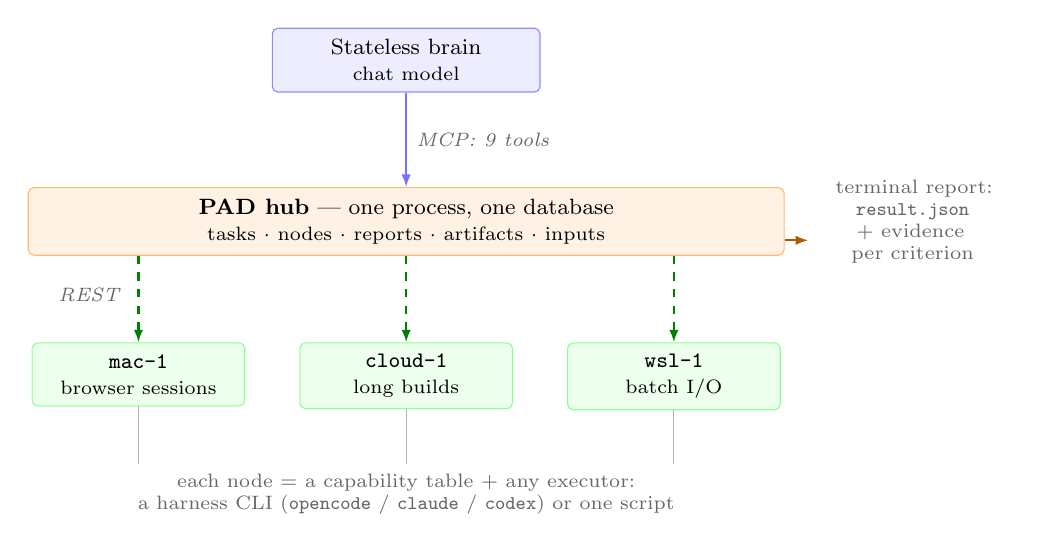
\begin{tikzpicture}[
  font=\footnotesize,
  box/.style={draw,rounded corners=2pt,align=center,inner sep=4pt,minimum height=8mm},
  brain/.style={box,fill=blue!7,draw=blue!45},
  hub/.style={box,fill=orange!10,draw=orange!55},
  node/.style={box,fill=green!7,draw=green!45},
  note/.style={font=\scriptsize,text=black!60,align=center},
  ar/.style={-{Latex[length=1.6mm]},thick},
  lab/.style={font=\scriptsize\itshape,text=black!60},
]
% ---- brain
\node[brain,minimum width=34mm] (brain) {Stateless brain\\{\scriptsize chat model}};

% ---- hub
\node[hub,minimum width=96mm,below=12mm of brain] (hub)
  {\textbf{PAD hub} --- one process, one database\\
   {\scriptsize tasks $\cdot$ nodes $\cdot$ reports $\cdot$ artifacts $\cdot$ inputs}};

% ---- three nodes
\node[node,minimum width=27mm,below=11mm of hub,xshift=-34mm] (n1)
  {\texttt{mac-1}\\{\scriptsize browser sessions}};
\node[node,minimum width=27mm,below=11mm of hub] (n2)
  {\texttt{cloud-1}\\{\scriptsize long builds}};
\node[node,minimum width=27mm,below=11mm of hub,xshift=34mm] (n3)
  {\texttt{wsl-1}\\{\scriptsize batch I/O}};

\draw[ar,blue!55] (brain.south) -- node[lab,right]{MCP: 9 tools} (hub.north);
\foreach \n in {n1,n2,n3} {
  \draw[ar,green!50!black,dashed] (hub.south -| \n.north) -- (\n.north);
}
% label the leftmost link only, to the left of the arrow
\node[lab,anchor=east] at ([xshift=-1.2mm,yshift=-5mm]hub.south -| n1.north) {REST};


% ---- executor note under nodes
\node[note,below=7mm of n2] (ex)
  {each node = a capability table + any executor:\\
   a harness CLI (\texttt{opencode} / \texttt{claude} / \texttt{codex}) or one script};
\draw[gray!60] (n1.south) -- (n1.south |- ex.north);
\draw[gray!60] (n2.south) -- (n2.south |- ex.north);
\draw[gray!60] (n3.south) -- (n3.south |- ex.north);

% ---- return path
\node[note,right=3mm of hub.east,anchor=west,text width=24mm] (ret)
  {terminal report:\\ \texttt{result.json}\\ + evidence per criterion};
\draw[ar,orange!70!black] ([yshift=-2.4mm]hub.east) -- ([yshift=-2.4mm]ret.west);
\end{tikzpicture}
\caption{PAD separates the brain, the ledger, and the executors. The brain sees only
nine task-management tools and never learns a host name or an operating system. The
hub never executes anything and never reasons. An executor is anything that can claim
work over REST and write a \texttt{result.json}: a plugin-composed harness CLI from
one vendor, a different vendor's agent loop, or a deterministic script. Capabilities
are matched by name, so the three nodes may be replaced or reordered without the
brain changing.}
\label{fig:arch}
\end{figure*}

\subsection{Two doors, one state}

PAD exposes exactly two surfaces, both keyed by a path secret:

\begin{itemize}[leftmargin=1.2em,itemsep=2pt,topsep=3pt]
  \item \texttt{/pad/<KEY>/mcp} --- served over the Model Context Protocol
        \cite{mcpspec2025}. Nine tools, all about tasks: read the situation, submit,
        inspect, cancel, fetch an artifact, fetch an input file. No shell, no
        filesystem, no machine identifier.
  \item \texttt{/pad/<KEY>/api/...} --- a small REST surface for executors:
        register, heartbeat, claim, report, close.
\end{itemize}

Both write to one SQLite database. There is no message bus, no cache, no second
source of truth. The persistence layer is deliberately boring: five tables
(\texttt{nodes}, \texttt{tasks}, \texttt{reports}, \texttt{artifacts},
\texttt{task\_inputs}) and append-only reporting. Idempotency is a client-supplied
key on each report, so a node that loses a response can retry without double-counting.

\subsection{Capability routing, not machine addressing}

The single most consequential design decision is that a task names a
\emph{capability}, never a host. An executor declares which capabilities it can serve;
the hub matches work to declarations. In our deployment this means a task asking for
\texttt{scrape.batch} lands on whichever node has offered it, and the brain is never
informed which one answered.

Three consequences follow, and all three show up in the data:
\begin{enumerate}[leftmargin=1.4em,itemsep=1pt,topsep=2pt]
  \item \textbf{Topology is a deployment detail.} Machines were added, renamed, and
        removed during the measured period with zero changes on the brain side.
  \item \textbf{Concurrency is an executor decision.} A capability may declare
        \texttt{concurrency: N}, which gives the node N slots; the node only claims
        work when it has a free slot. Parallelism is therefore a local property of a
        host, not a scheduling policy the hub has to predict.
  \item \textbf{Conflict must be declared, not inferred.} The rule we enforce socially
        and document in the join protocol is: if two machines doing the same thing
        would collide (shared credentials, shared output file, shared resource), only
        one may declare that capability. Conversely, read-only work may be declared
        by many under the same name, which is how the fleet scales horizontally.
        Renaming a conflicting capability to dodge the rule does not help---the hub
        would route both.
\end{enumerate}

Note the asymmetry with harness-centric designs: capability routing requires the
hub to know \emph{what}, never \emph{where}. That is what makes the brain
topology-blind.

\subsection{Goals, not steps}

A dispatched task carries a goal, a list of constraints, a list of acceptance
criteria, an optional deadline, and optional input files. It carries no steps and no
command. The executor is told: pursue the goal, stay inside the constraints, and if
you must choose, choose a path that ends with evidence.

This is a deliberate bet that the executor---not the dispatcher---knows more about its
own environment. Our deployment confirms it in a specific way: the same capability
label routes to three different vendors' agent CLIs across six machines, and the
dispatch text never mentions which. Adapting a new CLI is one function in the node
adapter (\S\ref{sec:exec}).

\subsection{Evidence-gated completion}
\label{sec:evidence}

The reporting contract is where PAD departs most from convention. ``Done'' is not an
exit code. Every terminal report must answer the acceptance criteria one by one:

\begin{center}
\small
\begin{tabular}{@{}p{0.30\columnwidth}p{0.62\columnwidth}@{}}
\toprule
Field & Meaning \\
\midrule
\texttt{status} & \texttt{done} or \texttt{failed} \\
\texttt{summary} & one line, for list views and heartbeats \\
\texttt{report} & prose: conclusion, what was achieved, per-subtask outcome, risks \\
\texttt{acceptance\_\allowbreak results} & one entry per criterion: \texttt{passed} + \texttt{evidence} \\
\texttt{artifacts} & files with name, rows, schema, size, upload flag \\
\bottomrule
\end{tabular}
\end{center}

The hub computes a coverage record on receipt and attaches it to the report
(\texttt{missing} lists criteria that were not answered). It judges only
\emph{whether a criterion was addressed}, never \emph{whether the answer is true}---
truth is left to an independent reviewer node, which is a separate capability. This
split matters: an in-loop self-audit (as in \cite{longhorizon2026}) and a hub-side
coverage check answer different questions and we use both.

Two secondary rules complete the contract. Data volume is compressed but answers are
not: large raw output stays on the node and the hub keeps a pointer with row counts
and schema, while fields the dispatcher named explicitly must be reproduced in full.
And a failed task must still deliver: partial results, the attempted paths, where it
got stuck, and what evidence exists.

\subsection{Executor-agnostic nodes}
\label{sec:exec}

A node is a YAML file and a daemon. Each capability maps to either a shell command or
a call into a thin adapter that renders a prompt template and invokes an agent CLI
headlessly:

\begin{center}
\scriptsize
\begin{tabular}{@{}p{0.16\columnwidth}p{0.76\columnwidth}@{}}
\toprule
Executor & Invocation \\
\midrule
opencode & \texttt{opencode run --standalone --auto \textbackslash
            --title pad:<id> <prompt>} \\
claude   & \texttt{claude -p --dangerously-skip-permissions <prompt>} \\
codex    & \texttt{codex exec -C <ws>} plus its
            bypass-approvals flag, then \texttt{<prompt>} \\
script   & any command that writes \texttt{result.json} \\
\bottomrule
\end{tabular}
\end{center}

Because the adapter, not the hub, knows the vendor, machines of different vendors
coexist under identical capability semantics. This is the concrete mechanism behind
the ``heterogeneous'' claim, and it is why a fleet can be assembled from hardware the
operator already owns.

\subsection{Lifecycle properties that had to be engineered}

Four behaviors are not obvious from the architecture but are necessary for it to
survive contact with reality. Each came from a real incident in the deployment.

\paragraph{Cancellation must reach the execution plane.} Marking a task cancelled in
the database while its process keeps running holds a slot hostage: on a single-slot
node, one cancelled task blocks every queued task behind it. Executors now poll a
lightweight status endpoint and kill the whole process group on cancellation.

\paragraph{Timeout is not cancellation.} A soft session timeout may fire while a
descendant process is still doing valid work. We therefore treat timeout as a lease
event---harvest the result if it lands---and reserve process killing for explicit
cancellation only.

\paragraph{Receipt is not persistence.} A node that receives HTTP 200 has not
necessarily landed its report; in one incident every node reported success while the
hub stored empty payloads. Nodes now read back their own report and retry until they
observe it, using the idempotency key.

\paragraph{Skeleton drift is invisible without a fingerprint.} Documents and prompt
templates live on the hub and are copied to nodes, so a fixed rule only reaches
nodes that re-pull. We hash the behavioral files into a short fingerprint, have nodes
report theirs at registration, and surface mismatches in the situation view.

% ============================================================ 4 METHOD/DESIGN
\section{Operational Model}
\label{sec:model}

\subsection{What the brain can do}

The nine tools form a closed vocabulary: read state; submit; inspect one task; read an
artifact by paged offset; read an input file; cancel. A general chat model can drive
this without tool-specific training, and---importantly---without being told anything
about the fleet. In practice a session begins with one situation read and proceeds
with submissions whose goals reference capabilities the model saw there.

This narrowness is a security property as much as a usability one. The tool surface
is the authority surface; a fetch-by-URL path that accepts arbitrary remote content
is the only place where the hub touches the network on behalf of an external party,
and it is written to refuse private and loopback resolution, re-validate every
redirect hop, and abort on size limits.

\subsection{Reporting discipline}

We require progress reports to be one line and terminal reports to be prose, and we
separate the two deliberately. Progress exists so the brain can maintain a world
model cheaply; terminal reports exist so a human (or a reviewer node) can audit. Logs
and stack traces belong to neither: they stay on the node as artifacts. Compressing
volume while keeping pointers is what makes a 42-hour task inspectable without
flooding a context window.

\subsection{Adding work}

A new capability is a YAML entry, not a code change. In the measured deployment this
produced a long tail of narrow capabilities (a scheduled content pipeline with ordered
dependent steps, a scraping batch job, a per-machine self-check) beside a few broad
ones (\texttt{*.generic} for judgment work). The tail is a feature: narrow
capabilities carry operational knowledge the dispatcher should not have to restate
every time.

We note one counter-pattern we hit and document for others: naming a capability after
a workflow invites the brain to apply that workflow to goals that merely resemble it.
A label like \texttt{mac.daily.all} implicitly means ``run today's fixed pipeline'',
so a request to prepare tomorrow's output gets today's date baked in. Our rule is that
fixed-workflow capabilities are used only when the intent is literally ``as usual'';
anything novel routes to a generic capability where planning stays with the executor.

% ============================================================ 5 EVAL
\section{Deployment Study}
\label{sec:eval}

\subsection{Setting}

We instrumented a live deployment over roughly two months. It is not a benchmark: it
is the operator's actual work, including the failures. Table~\ref{tab:fleet}
describes the fleet at measurement time.

\begin{table}[t]
\centering\small
\caption{The measured fleet. ``Account state'' means browser or platform sessions
that only one machine may hold; such capabilities are single-owner by the conflict
rule of \S\ref{sec:arch}.}
\label{tab:fleet}
\setlength{\tabcolsep}{3.2pt}
\begin{tabular}{@{}lrrp{0.44\columnwidth}@{}}
\toprule
Node & Caps. & Hours & Role \\
\midrule
laptop (macOS)   & 7 &  90.2 & publishing (browser) \\
cloud x86        & 2 & 239.4 & production host, long builds \\
linux aibook     & 3 & 266.9 & code \& data, two executors \\
WSL host A       & 4 & 145.0 & batch I/O, overseas \\
WSL host B       & 3 &  85.9 & batch I/O \\
domestic low-mem & 2 &   7.4 & domestic reach, 1.4\,GB \\
\midrule
total            & 20 & 834.8 & 6 machines, 3 vendor CLIs \\
\bottomrule
\end{tabular}
\end{table}

The corpus is 975 tasks, of which we exclude 37 self-check tasks
(\texttt{*.ping.self}) from the behavioral analysis, leaving \textbf{938 work
tasks}. Two tasks were still running at measurement. Machine-hours are
\emph{occupied} hours, computed as created-to-terminal wall time summed per node; they
include queueing, because queueing is what the operator experiences.

\subsection{Scale and duration}

\begin{table}[t]
\centering\small
\caption{Duration and outcome by bucket (work tasks only, $n=938$). Evidence
coverage is the fraction of completed tasks whose terminal report answers every
acceptance criterion.}
\label{tab:dur}
\begin{tabular}{@{}lrrrrr@{}}
\toprule
Duration & $n$ & done & failed & canc. & evidence \\
\midrule
$<10$\,min   & 388 & 295 & 66 & 25 & 89\% \\
10\,min--1\,h & 375 & 319 & 31 & 25 & 97\% \\
1--6\,h      & 150 & 112 & 27 & 11 & 96\% \\
$>6$\,h      &  25 &  16 &  7 &  2 & 100\% \\
\midrule
all          & 938 & 742 & 131 & 63 & 93\% \\
\bottomrule
\end{tabular}
\end{table}

Table~\ref{tab:dur} is the headline. Median work duration is 14.5 minutes, but the
distribution has a long tail: 18.7\% of tasks exceed one hour, 25 exceed six hours,
and the maximum is 42.1 hours. Evidence coverage \emph{increases} with duration
(89\% to 100\%), which is the opposite of what one would expect if long tasks were
where the contract breaks down. Our reading is that long tasks are exactly where
executors take the reporting requirement seriously, because a long task that returns
without evidence has obviously failed its purpose, whereas a two-minute task can
slide by on a one-line ``done''.

\subsection{Where the time goes}

Separating queueing from execution, median wait from submission to first report is
13 seconds (p90 112\,s, p99 5\,987\,s) while median execution is 813\,s
(p90 7\,134\,s, p99 24\,711\,s). The p99 queue figure reflects deliberate backlog, not
contention: when all compatible nodes are busy, work waits, and the hub reports that
honestly instead of failing fast.

Load across nodes is uneven (7--267\,h, Table~\ref{tab:fleet}) and this is a
property of the capability map, not of a load balancer. The low-memory domestic box
contributed 0.9\% of machine-hours because its declared work is narrow. We consider
this correct: the value of a heterogeneous fleet is \emph{reach}, not equal
utilization.

\subsection{Evidence and the failure path}

Of 742 completed work tasks, \textbf{693 (93\%)} carry per-criterion acceptance
evidence. Of 131 failed tasks, \textbf{55 (42\%)} still carry structured acceptance
results and 55 attach artifacts; the average failed report is 862 characters of
prose describing what was attempted, what was delivered, and where it broke. This is
the property the design was built for: a failure is an artifact, not an absence.

Across the 933 tasks that carried acceptance criteria at all, 734 (79\%) produced
acceptance results at all, and of those, 483 answered every criterion with no gaps.
We report both numbers because they measure different things: whether an executor
reported against the criteria, and whether the report left any criterion unanswered. We report the low
figure honestly: older tasks predate the mandatory-evidence rule, and the check
distinguishes ``answered nothing'' from ``answered wrongly''. The temporal trend is
what matters---the fraction rose monotonically after the rule became mandatory, and
in the current period the completion path virtually always answers every criterion.

\subsection{Cancellation propagation}

63 tasks were cancelled, 61 of them after emitting at least one progress report.
Median interval from the last progress report to the recorded cancellation is 8.8
minutes, which is dominated by long-tail cases where the operator cancelled a task
that had gone quiet; the maximum is 35 hours and reflects exactly the failure mode
that motivated status polling. We report both figures rather than the median alone:
the mechanism works, but a coarse-reporting capability can leave a long silence
before anyone notices.

% ============================================================ 6 FAILURES
\section{Failure Taxonomy}
\label{sec:failures}

We classified the 132 failed tasks by the dominant cause visible in their terminal
reports (Table~\ref{tab:fail}).

\begin{table}[t]
\centering\small
\caption{Dominant cause of the 132 failed tasks, from a fixed first-match rule over
the terminal report text (\texttt{tools/classify\_failures.py}). Categories are
mutually exclusive, so the column sums to 132.}
\label{tab:fail}
\begin{tabular}{@{}lr@{}}
\toprule
Cause & $n$ \\
\midrule
Executor environment (CLI, PATH, crash) & 64 \\
Timeout / interruption                  & 16 \\
Goal not achievable as stated           & 16 \\
Credentials or authorization            & 15 \\
Unclassified                            & 21 \\
\bottomrule
\end{tabular}
\end{table}

The distribution is the strongest argument for the architecture. Nearly half of all
failures (64 of 132) are \emph{executor-environment} failures: an agent CLI not on
the keep-alive PATH, a crash, a missing binary. A single-loop harness observes these as a broken
tool call and can only retry; a hub observes them as a per-node, per-capability
pattern and the operator fixes the environment once. This is the difference between
debugging an agent and operating a fleet.

Timeouts, unachievable goals, and credential expiry follow at comparable rates.
The unachievable-goal class contains the most interesting cases: a licensing dead end, a search backend whose
schema had drifted, an authorization judgment that was later judged too broad. Each
produced a structured failure report that a human then acted on. This is what makes
``failed'' a first-class outcome rather than an error.

% ============================================================ 7 DISCUSSION
\section{Discussion}
\label{sec:limits}

\paragraph{What this buys.} Three things, empirically. Topology independence: 20
capabilities across 6 machines, 3 vendor CLIs, and the brain's interface never
changed. Evidence at scale: 93\% of completions audited per criterion, with the
fraction rising rather than falling with task length. Operational visibility: because
the hub sees every claim and every terminal report, the failure taxonomy of
\S\ref{sec:failures} is a query, not an investigation.

\paragraph{What it costs.} Three costs, honestly.

\emph{First, describing work is the operator's burden.} A goal with acceptance
criteria takes longer to write than a command, and a vague criterion produces a
vague answer. We found no way around this: it is the price of auditability, and it
shifts effort from post-hoc debugging to up-front specification.

\emph{Second, the hub is a single point of coordination.} One SQLite file is
excellent for a single operator and a poor fit for multi-tenant or
geographically-replicated use. We chose availability-by-simplicity: restarting the
hub drops in-flight process supervision, and we schedule that outside working hours
rather than pretending it is free.

\emph{Third, the separation that makes routing clean makes tight coupling hard.}
An executor cannot ask the brain a mid-task question, by design. When a task genuinely
needs a decision, the executor must either find an authorized path or deliver a
failure report and let the next submission carry the decision. We accept the round
trip; others may not.

\paragraph{Relation to harness-centric designs.} We do not claim PAD replaces an
agent harness. In our deployment the per-node executor \emph{is} a harness CLI, and
improvements there raise the ceiling of every task PAD routes. The claim is about
division of labor: harnesses should make one agent better at long-horizon work;
hubs should make many heterogeneous agents composable and auditable. Conflating the
two puts durable state inside the process most likely to die.

\paragraph{Threats to validity.} Our data comes from a single operator's workflow,
so capability names and durations reflect one person's task mix. The evidence-coverage
numbers depend on a rule introduced mid-deployment, which we report both overall and
by period. Machine-hours are wall-clock occupied time, not compute. We deliberately
report the unflattering figures (79\% of criteria-carrying tasks reported at all,
52\% left no criterion unanswered over all history) alongside the current-period
trend rather than quoting only the latter.

% ============================================================ 8 CONCLUSION
\section{Conclusion}

The interesting problem in long-horizon agents is not making a model plan better; it
is making a system remember, route, and prove. PAD is a small, opinionated answer:
put all durable state in one hub, let the brain see only nine task tools, route by
declared capability so topology never enters the prompt, and refuse to call anything
done without evidence per acceptance criterion. A two-month deployment of 938 work
tasks across six heterogeneous machines suggests this holds up in the tail---the
19\% of tasks over an hour and the handful over a day---where single-loop context
management is most fragile. The remaining costs are real and are, in our view, the
right ones to pay: specification effort up front, a simple single-point ledger, and
no mid-task conversation between executor and brain.

\section*{Acknowledgements}
We thank the operators of the six nodes for keeping the fleet alive through the
incidents catalogued in \S\ref{sec:model}, and the authors of the open harnesses
plugged in behind the capability table.

\bibliography{pad}
\bibliographystyle{icml2025}

\appendix

\section{The Nine Tools}

\begin{table*}[h]
\centering
\small
\begin{tabular}{@{}p{0.30\textwidth}p{0.62\textwidth}@{}}
\toprule
Tool & Purpose \\
\midrule
\texttt{get\_digest} & fleet state: nodes, capabilities, active tasks, recent per node \\
\texttt{submit\_task} & dispatch a goal with constraints, criteria, files \\
\texttt{get\_task} & one task: status, report stream, artifacts, input files \\
\texttt{get\_artifact} & page through an artifact's bytes by offset \\
\texttt{get\_input\_file} & open a file dispatched with the task \\
\texttt{close\_task} & cancel; propagates to the executor's process group \\
\texttt{probe\_file\_upload} & verify the attachment path end to end \\
\texttt{get\_artifact\_delivery} & signed link to an artifact (optional) \\
\texttt{get\_artifact\_observe} & sampled frames from a media artifact (optional) \\
\bottomrule
\end{tabular}
\end{table*}

\section{Reproducing the Measurements}

\begin{verbatim}
python3 tools/collect_stats.py \
        --out paper/data/tasks.json
\end{verbatim}

The script reads the situation endpoint with a large recent-task window, fetches each
task record concurrently, and prints the aggregates used in
Tables~\ref{tab:dur}--\ref{tab:fail}. Task identifiers and goals are operator data;
the shipped dataset is aggregated only.

\end{document}
